\documentclass[11pt]{article}
\usepackage[margin=1in]{geometry}
\usepackage{graphicx}
\usepackage{amsmath}
\begin{document}
\section*{R97 finite discriminant locus of the marked-23 base}
The frozen producer and corrected fresh-readback replay agree on the
exact degree-7 base-order resultant
\[
\operatorname{Res}_y(f_{23},\partial_y f_{23})
=x^{22}(x+1)^{14}(x^7+x^6+x^3+x+1)^2.
\]
The factor degree contributions are 22, 14 and 14, totaling 50.

\begin{center}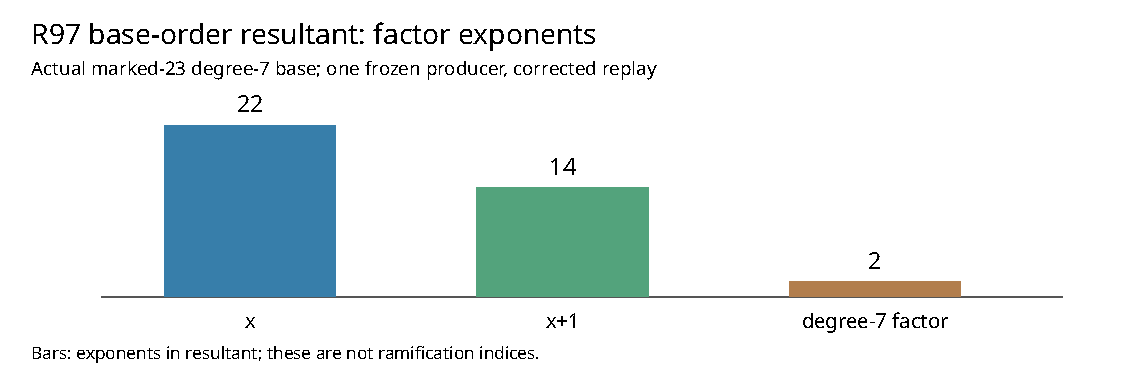
\includegraphics[width=.88\textwidth]{diagram.pdf}\end{center}

The strict producer had native exit zero and no errors. The first
replay was rejected for an identifier collision despite a late marker;
the corrected replay was pushed before execution and passed without
errors. All 16 raw members passed fresh S3 readback hashes. The three
factor supports locate finite fibers where the monogenic base order
can fail to be etale. Normalized branches and the full degree-112
lambda-extension discriminant remain separate calculations.
\end{document}
